%\documentclass[12pt,preprint]{aastex6}
%\documentclass[manuscript]{aastex6}
%\documentclass{emulateapj}
\documentclass[12pt]{revtex4}
%\usepackage{esvect}
\usepackage{amsmath}
\usepackage{amssymb}
\usepackage{graphicx}
\usepackage{color}
\DeclareMathOperator{\csch}{csch}
%\shorttitle{Schwinger in De Sitter}
%\shortauthors{Haider, Fertig, \& Bonga}

\newcommand{\red}{\textcolor{red}}
\newcommand{\blue}{\textcolor{blue}}



\begin{document}
	
	\begin{titlepage}
		\title{Schwinger Effect in De Sitter Space}
		
		\author{J. Haider, A. Fertig, \& B. Bonga}
		
		\affiliation{Perimeter Institution for Theoretical Physics}
		
		\email{syedjibran.haider@richmond.edu}
		
		
		\begin{abstract}
			Electric fields as well as gravitational fields can create pairs of particles via quantum tunneling (the Schwinger mechanism [1,2]). These processes are usually studied using quantum field theory on Minkowski or curved space-times. There is an alternative to Feynman diagram loop calculations -- the worldline formalism --, which can offer insights into the space-time evolution of the produced particles.
			When the solutions of the classical equations of motion are known, the path integral in the quantum mechanical propagator is reduced to an ordinary integral over the internal time of the particle. We can then study the semiclassical limit using Picard-Lefschetz theory [3], a set of mathematical tools for oscillatory integrals, which has given exciting new results in recent years (in quantum cosmology, QCD lattice computation, non-perturbative quantum field theory). 
			The goal of the project is to apply Picard-Lefschetz theory to pair production in de Sitter space-time (with or without a constant electric field [4]). The process, besides being interesting in itself, could help model pair production in black holes, bubble nucleation, or the production of universes.
			
		\end{abstract}
	\maketitle
	\end{titlepage}

\tableofcontents
\newpage

\section{Background Information} \label{background}
Before diving fully into the project, i.e. to look at the Schwinger effect in de Sitter space-time, I will begin by first working with the Schwinger effect in electric fields to make acquaintance with the fundamental processes that will be studied throughout the project. In order to do that, there is a further need to establish some foundational physical and mathematical concepts, viz. Einstein notation (along with tensors and the metric), field dynamics, Lorentz transformations, Lagrange multipliers, gauge fixing, Feynman path integral formalism, and ADM formalism.

\subsection{Einstein Notation \& the Metric} \label{einstein}
In Euclidean space (Cartesian coordinates), the invariant squared distance is represented by $\vec{a}^2=a_x^2 + a_y^2 + a_z^2$, where $\vec{a}=(a_x,a_y,a_z)$. Using index notation, we could write this as:
\[ \vec{a}^2 = \sum_{i=1}^{3} a_ia_i\]
where $a_i$ denotes each component of the vector, with $i=1,2,3$.

Similarly, in relativity we have 4-component vectors in space-time, but here we use Greek letters to represent indices. So, a 4-vector would then be $a^\mu=(ca_t,a_x,a_y,a_z)$, with $\mu=0,1,2,3$. Note that $a^\mu$ represents the full vector component-wise. 

Why do we need to use this notation, called Einstein notation, among other names, in order to talk about vectors in space-time? The need arises due to the geometry of Minkowski space, i.e. the geometry of space-time, which has the usual three Euclidean space coordinates along with an additional time coordinate, and how the Minkowskian geometry defines the invariant squared `distance' in Minkowski space. This invariant squared distance is $-(ca_t)^2+a_x^2+a_y^2+a_z^2$. Notice how we were easily able to represent the invariant squared distance in Euclidean space merely by squaring a Euclidean vector. We can't, however, do the same in Minkowski space since we have a minus sign with just the first term, and simply squaring a 4-vector would not return such an invariant line element. Einstein (index) notation helps us overcome this issue by allowing us to differentiate between different vectors and their components in a subtle manner. Briefly, then, we can extract the invariant line element by doing the following:
\[ a^\mu a_\mu \equiv \sum_{\mu=0}^{3} a^\mu a_\mu\]
where $a^\mu=(ca_t,a_x,a_y,a_z)$ and $a_\mu\equiv(-ca_t,a_x,a_y,a_z)$. The negative signs can be moved around, as some authors do, as long as the final invariant line element remains the same. Regardless, it is not defined to multiply two vectors together in this notation if both are `up' or `down' (in terms of how their indices are placed). To be specific, the `up' indexed vectors are called contravariant, and the `down' indexed covariant. Finally, note that the summation is implied without the sum sign.

In general relativity, when one generalizes to possibly curved 4-D space-times, Minkowski space must then also be generalized. In that case we have to introduce the \textit{metric} $g_{\mu\nu}$. The metric is a rank 2 tensor, i.e. a 2-D matrix. Since it has Greek letter indices we know it is 4x4 in size (one Greek index representing each dimension). When considering the metric, one must utilize operations from linear algebra, such as matrix multiplication.
For the special case of flat Minkowski space, for example, the metric is
\[ g_{\mu\nu} = \begin{pmatrix}
-1 & 0 & 0 & 0 \\ 
0 & 1 & 0 & 0 \\ 
0 & 0 & 1 & 0 \\ 
0 & 0 & 0 & 1
\end{pmatrix} \]

One can think of $\mu=0,1,2,3$ and $\nu=0,1,2,3$ indexing the rows and columns. For a symmetric metric, $\nu$ and $\mu$ are interchangable, so it is not so much that one of them corresponds to the rows and one to the columns as that the presence of both indicates that there are both rows and columns, i.e. that it is a matrix. However, for a general tensor, the indices are not interchangable. If there was only one Greek letter index then it would indicate a vector.

Observe, then, that using matrix multiplication,
\[ g_{\mu\nu}a^{\nu} = \begin{pmatrix}
-1 & 0 & 0 & 0 \\ 
0 & 1 & 0 & 0 \\ 
0 & 0 & 1 & 0 \\ 
0 & 0 & 0 & 1
\end{pmatrix} \begin{pmatrix}
ca_t \\ 
a_x \\ 
a_y \\ 
a_z 
\end{pmatrix} = \begin{pmatrix}
-ca_t \\ 
a_x \\ 
a_y \\ 
a_z 
\end{pmatrix} = a_{\mu} \]

The result is a covariant (down index) vector because there is a minus sign in the 0-component. Then the vector product $a^{\mu}a_{\mu}$ can be expressed in terms of only contravariant (up index) 4-vectors and the metric:
\[ a^{\mu}a_{\mu}= a^{\mu}g_{\mu\nu}a^{\nu} \]

Again, note that \textit{repeated indices are always summed or ‘collapsed’ over, and any summing or collapsing must have one up index and one down index}. It is simply not defined to have $a^{\mu}a^{\mu}$ (ultimately this derives from the need to preserve a negative in the square of a 4-vector, as seen above). Also, it is important to keep in mind that a Greek letter solely indicates that there are four components. $a^{\mu}$ is no different than $a^{\nu}$ – both represent a vector with four components.

There would also be a contravariant metric $g^{\mu\nu}$ such that $g^{\mu\nu}g_{\mu\nu}= \mathbb{I}_4$ where $\mathbb{I}_4$ is the 4x4 identity matrix. Then $g^{\mu\nu}a_{\nu}=a^{\mu}$. In this way we speak of the metric “raising and lowering indices.”

In a general curved spacetime the metric will be not a simple diagonal as above and would then “mix” the different components of 4-vectors when acting on them. It gets difficult to visualize and write all that out which is why Einstein notation is so useful [6].

\subsection{Field Dynamics} \label{field}
Let us derive the Klein-Gordon equation, as a sample problem of working with Einstein notation, using Lagrangian mechanics as applied on fields instead of particles. In order to do so, we first need to establish a different form of the Euler-Lagrange equation to describe the dynamics of a field.  Note that since we desire to draw a parallel between regular vector notation and Einstein notation, we will write down equations, or at least elaborate on the interpretation of specific elements of equations, using both notations at each step. 

The first step involves introducing the form of the action, but instead of starting with the Lagrangian, we start with the Lagrangian density, which is the Lagrangian per unit spatial volume. For a Lagrangian that depends on the field, $\phi(\vec{x},t)$, its time derivative, $\dot{\phi}(\vec{x},t)$, and its gradient, $\nabla \phi (\vec{x},t)$, we get
\[ L(t)=\int d^3 x \, \mathcal{L}(\phi,\partial_{\mu}\phi),\]
where $x$ is any of the three spatial dimensions, $\mathcal{L}$ is the Lagrangian density, and $\partial_{\mu} \phi = (\dot{\phi},\nabla\phi)$ is the four-gradient (i.e. the four-vector analogue of the gradient operator). Notice that the four-gradient allows the consolidation of the time derivative and gradient dependence of the Lagrangian because we are dealing with Minkowski space. The action is thus given by,
\[ S = \int_{t_1}^{t^2}dt \, \int d^3 x \, \mathcal{L} = \int d^4 x \mathcal{L},\]
where $x$ is now representative of all four coordinates of spacetime.

Employing the principle of least action,
\begin{equation} \label{leastaction}
\delta S = \int d^4 x \, \delta \mathcal{L} = 0.
\end{equation}
Here, the Lagrangian (density) is dependent on $\phi$ and $\partial_{\mu} \phi$, thus
\[ \delta \mathcal{L} = \frac{\partial \mathcal{L}}{\partial \phi} \delta \phi + \frac{\partial \mathcal{L}}{\partial (\partial_{\mu} \phi)} \delta (\partial_{\mu} \phi)\]
Plugging this back into Eq. \ref{leastaction} returns:
\begin{align*}
\delta S &= \int d^4 x \, [\frac{\partial \mathcal{L}}{\partial \phi} \delta \phi + \frac{\partial \mathcal{L}}{\partial (\partial_{\mu} \phi)} \delta (\partial_{\mu} \phi)] \\
&= \int d^4 x \, [\frac{\partial \mathcal{L}}{\partial \phi} - \partial_{\mu}(\frac{\partial \mathcal{L}}{\partial (\partial_{\mu} \phi)})]\delta \phi + \partial_{\mu}(\frac{\partial \mathcal{L}}{\partial (\partial_{\mu} \phi)}\delta \phi)\end{align*} 
Since $\delta \phi = 0$ at the end points, the last term, which is a total derivative, disappears. This necessitates the following condition:
\[ \partial_{\mu}(\frac{\mathcal{L}}{\partial(\partial_{\mu}\phi)}) - \frac{\mathcal{L}}{\partial \phi} = 0\]
which is the Euler-Lagrange equation for a field $\phi$.

Now, having ascertained the Euler-Lagrange equation, the equations of motion can be determined by using the Lagrangian density for a real scalar field $\phi (\vec{x},t)$,
\[ \mathcal{L} = \dfrac{1}{2} \eta^{\mu\nu} \partial_{\mu} \phi \partial_{\nu} \phi - \dfrac{1}{2}m^2\phi^2,\]
using the (+ - - -) Minkowski space metric signature. In regular vector notation, the Lagrangian density can be written as,
\[ \mathcal{L} = \dfrac{1}{2} \dot{\phi^2} - \dfrac{1}{2}(\nabla \phi)^2 - \dfrac{1}{2}m^2\phi^2.\]

We know that the Lagrangian $L=T - V$, where $T$ is the kinetic term and $V$ is the potential term. In our case,
\[ T = \int d^3 x \, \frac{1}{2} \dot{\phi}^2 \]
and,
\[ V = \int d^3 x \, \frac{1}{2} (\nabla \phi)^2 + \frac{1}{2}m^2 \phi^2.\]
In the expression for the potential energy, the first term is generally called the gradient energy and the second term the potential energy.

In order to determine the equations of motion, we need to solve the Euler-Lagrange equation by first computing,
\[ \frac{\partial \mathcal{L}}{\partial \phi} = -m^2 \phi \text{  and  } \frac{\partial \mathcal{L}}{\partial (\partial_{\mu} \phi)} = \partial^{\mu}\phi \equiv (\dot{\phi},-\nabla\phi)\]

Finally, putting our results together:
\[ \partial_{\mu}\partial^{\mu}\phi + m^2 \phi = 0 .\]
Or equivalently, in regular vector notation,
\[ \ddot{\phi} - \nabla^2\phi + m^2 \phi = 0. \]

\subsection{Lagrange Multipliers} \label{multpliers}
Lagrange multipliers are employed in the method of Lagrange multipliers that allows the optimization (i.e.~finding minima and maxima) of a function $f(x,y,z)$ subject to a constraint given by $g(x,y,z)=k$. The method involves solving the following:
\begin{align*}
	\nabla f(x,y,z) &= \lambda \nabla g(x,y,z) \\
	g(x,y,z)&=k
\end{align*}
where $\lambda$ is the Lagrange multiplier. Having solved the above equations, all solutions $(x,y,z)$ are plugged into $f(x,y,z)$ to identify minimum/maximum values, if they exist. 

\subsection{Feynman Path Integrals} \label{feynman}
Without going into the details of fundamental ideas of quantum mechanics, we note that for a given particle, there is a probability amplitude $\phi$ associated with each of the particle's trajectories (or, to generalize, with each of the specific events that are associated with anything in nature), where the square of the probability amplitude gives us the probability of the particle taking a particular trajectory. Given various alternative trajectories the particle can take from an initial point $a$ to a final point $b$, the sum of the amplitudes for each alternative trajectory returns an amplitude that can be associated with the overall trajectory from $a$ to $b$. The absolute square of the overall amplitude returns to us the probability of the particle reaching $b$ from $a$. Such an overall amplitude for an event is also called the \textit{kernel}, which may be given as $K(b,a)$ for the trajectory in our case. In contrast, classical mechanics asserts the existence of a single, unique trajectory for a particle going from $a$ to $b$. 

We know how the principle of least action can be employed in Lagrangian mechanics to describe the behavior of a particle, so let's take a look at the quantum-mechanical formalism. So far we have talked about the amplitude without talking about what it actually is for each alternative trajectory, which is exactly what we need to determine in order to devise the sum of the amplitudes of all possible trajectories. It turns out that each trajectory of a particle contributes equally in terms of magnitude, but does so at different phases. The overall amplitude of the trajectories from $a$ to $b$ is given by:
\[ K(b,a) = \sum_{\text{paths from $a$ to $b$}} \phi [x(t)] \]
and the contribution of each path to the amplitude is given by:
\[ \phi [x(t)] = k \; e^{(i/\hbar)S[x(t)]}, \]
where $k$ is a normalization constant and $S$ is the action associated with the corresponding classical system. More precisely, the overall amplitude can be defined as:
\[ K(b,a) = \int_{a}^{b}\mathcal{D}x(t) \; e^{(i/\hbar)S[b, a]} , \]
where $\mathcal{D}x(t)$ denotes the fact that we are integrating over all paths. This form is called the path integral.

Phase differences between alternative trajectories cause constructive and destructive interference between them, and it is the classical limit of this interference (i.e. when $S$ is much bigger than $\hbar$) that results in the classical path. That is, for the particular trajectory that the particle would take in the classical case, with minimum action, the phase changes infinitesimally with an infinitesimal change in the trajectory. These slightly different trajectories around the classically predicted trajectory will interfere constructively, whereas elsewhere, slight changes in the trajectory result in substantial changes in the phase such that their contributions to the amplitude will cancel out. Ultimately, this yields the classically predicted particular trajectory as the behavior of significance. In the semi-classical approximation, the kernel can thus be expressed in the form:
\begin{equation} \label{sckernel}
K(b,a)=\text{``smooth function''}\cdot e^{iS_{\rm cl}/\hbar}
\end{equation} 
where $S_{\rm cl}$ knows about the boundary conditions $a$ and $b$.

\subsubsection{Example: Harmonic Oscillator}
For a harmonic oscillator, the Lagrangian is:
\[ L = \frac{m}{2}\dot{x}^2 - \frac{m \omega^2}{2}x^2 \]
We need to determine the equations of motion and solve them for $x(t)$ in order to find the classical action. The Euler-Lagrange equation gives us:
\begin{equation*}
\frac{d}{dt}\frac{\partial L}{\partial \dot{x}}-\frac{\partial L}{\partial x} = m\ddot{x}+m\omega^2x=0
\end{equation*}
The equation of motion is a differential equation, which can be solved to get $x(t)$ with the boundary conditions $x(0) = x_a$ and $x(T)=x_b$, where $T=t_b-t_a$, and $t_b$ is the final time and $t_a$ is the initial time, which we set equal to zero. This returns:
\[ x(t)= x_a \cos(t\omega) - x_a \cot(T \omega)\sin(t \omega)+x_b\csc(T \omega)\sin(t \omega) \]

Plotting the position $x$ with respect to time $t$ after defining the parameters yields the typical sinusoidal trajectory of a harmonic oscillator. This is illustrated in Fig.~\ref{fig:oscillator}.

\begin{figure}[h]
	\centering
	\includegraphics[width=0.7\linewidth]{"oscillator trajectory"}
	\caption{Red curve: $x_a=2$, $x_b=4$, $\omega=1$, $m=1$, and $T=1$. Green curve: $x_a=0$, $x_b=4$, $\omega=1$, $m=1$, and $T=1$.}
	\label{fig:oscillator}
\end{figure}

Substituting the solution for $x(t)$ into the action, the classical action for the boundary conditions specified above is: 
\begin{align*}
S &= \int_{0}^{T} \frac{1}{2} m (-x_a \omega \cos(t \omega) \cot(T \omega) + 
x_b \omega \cos(t \omega) \csc(T \omega) - 
x_a \omega \sin(t \omega))^2 - \\
&\qquad \frac{1}{2} m \omega^2 (x_a \cos(t \omega) - 
x_a \cot(T \omega) \sin(t \omega) + 
x_b \csc(T \omega) \sin(t \omega))^2 \\
&=\frac{1}{2} m \omega (-2 x_a x_b + (x_a^2 + x_b^2) \cos(T \omega)) \csc(T \omega) \; .
\end{align*} 

In the semiclassical limit, using Equation \ref{sckernel}, the kernel can be expressed as 
\[ K(0,x_a;T,x_b)=F(T) \exp \Bigg[{\Bigg\{\frac{im\omega}{2 \hbar \sin\omega T} [-2 x_a x_b + (x_a^2 + x_b^2) \cos \omega T]\Bigg\}}\Bigg],\]
where $F(T)$ is the ``smooth function'', or the `prefactor', and needs to be found [5]. 

\subsubsection{Another Example: Relativistic Particle in Electric Field}
For a charged relativistic particle in an electric field, with motion restricted to just one spatial coordinate $x$, the Lagrangian is:
\[ L = \frac{m (-t'(T)^2 + x'(T)^2)}{2N} -\frac{m N}{2} + k x(T) t'(T),\]
where $N$ is the lapse, and $k$ is the strength of the electric field in positive $x$-direction times the charge of the relativistic particle. Note that the metric signature being used here is (- + + +).
\red{\\
Add comment about the choice of Lagrangian? (Classically yield the same equations of motion (provided that $dL/dT =0$ when evaluated on an eom; which is the case here), but the \textit{quantum} theories are different! 
However, given that we work in the semi-classical approximation the predictions with either Lagrangian should be similar.)
Typical choice is:
\begin{align}
 	L = - m \sqrt{\eta_{\mu \nu} \dot{x}^{\mu} \dot{x}^{\nu} } + e \; A_\mu \dot{x}^{\mu} 
\end{align}
Here, we used:
\begin{align}
L = \frac{m}{2} \sqrt{\eta_{\mu \nu} \dot{x}^{\mu} \dot{x}^{\nu} } + e \; A_\mu \dot{x}^{\mu} 
\end{align}
with $A_\mu = E_0 \; x \; \nabla_\mu t$ with $E_0$ a constant and $k := e E_0$.
\\
Also, since we reparametrized this path from some parameter $\tau$ to $T$ you should include this transformation (and find the factors of $N$ above).
}

We need to determine the equations of motion and solve them for $x(T)$ and $t(T)$ in order to find the classical action. The Euler-Lagrange equation gives us:
\begin{align*}
\frac{d}{dt}\frac{\partial L}{\partial x'}-\frac{\partial L}{\partial x} &= -k t'(T) + \frac{m x''(T)}{N} =0\\
\frac{d}{dt}\frac{\partial L}{\partial x'}-\frac{\partial L}{\partial t} &= k x'(T) - \frac{m t''(T)}{N} =0
\end{align*}
The equations of motion are a system of differential equation, which can be solved to get $x(T)$ and $t(T)$ with the simplified boundary conditions $x(0) = x_a = 0$, $x(1)=x_b$, $t(0) = t_a = 0$, and $t(1)=t_b$, where $x_b$ and $t_b$ are the final space-time coordinates and $x_a$ and $t_a$ are the initial space-time coordinates. This returns:
\begin{align*}
x(T) &= \csch \bigg(\frac{k N}{2 m}\bigg) \Biggr(x_b \cosh\bigg(\frac{k N (T-1)}{2m}\bigg)+ 
t_b \sinh\bigg(\frac{k N (T-1)}{2m}\bigg)\Biggr) \sinh\bigg(\frac{k N T}{2m}\bigg)\\
t(T)&= \csch \bigg(\frac{k N}{2 m}\bigg) \Biggr(t_b \cosh\bigg(\frac{k N (T-1)}{2m}\bigg)+ 
x_b \sinh\bigg(\frac{k N (T-1)}{2m}\bigg)\Biggr) \sinh\bigg(\frac{k N T}{2m}\bigg)
\end{align*} 

Plotting the time-coordinate $t(T)$ with respect to the spatial-coordinate $x(T)$ after defining and varying the parameters yields insightful graphical information (insert plot here - which one?).

\begin{figure}[h]
	\centering
	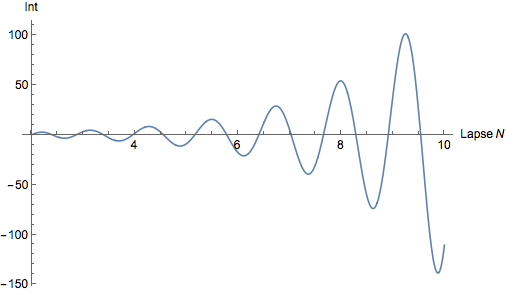
\includegraphics[width=0.7\linewidth]{integrandplot}
	\caption{Long caption}
	\label{integrandplot}
\end{figure}


For the given boundary conditions, with the solutions for $x(T)$ and $t(T)$ plugged in, and integrating the Lagrangian over $T$ from 0 to 1, the classical action  is:
\begin{equation*}
S_{\rm cl} = \frac{1}{4} \Bigg(-2 (m N - k t_b x_b) - k (-t_b - x_b) (-t_b + x_b) \coth\bigg(\frac{k N}{2 m}\bigg)\Bigg) \; .
\end{equation*} 

In the semiclassical limit, the kernel can then be expressed as 
\[ K=\int_{0}^{\infty} dN\ F(\red{N}) \exp \Bigg[\frac{i}{4 \hbar} \Bigg(-2 (m N - k t_b x_b) - k (-t_b - x_b) (-t_b + x_b) \coth\bigg(\frac{k N}{2 m}\bigg)\Bigg)\Bigg],\]
where $F(N)$ is the ``smooth function'', or the `prefactor', which we known to be of the form: $\frac{1}{\sqrt{Det(M)}}$, where $M$ is the following matrix:
\[ M=\begin{pmatrix}
\frac{\partial^2 S}{\partial x_a \partial x_b} & \frac{\partial^2 S}{\partial x_a \partial t_b} \\ 
\frac{\partial^2 S}{\partial t_a \partial x_b} & \frac{\partial^2 S}{\partial t_a \partial t_b} 
\end{pmatrix} = 
\begin{pmatrix}
-\frac{k}{2}  \coth(\frac{k N}{2 m}) & \frac{k}{2} \\ 
-\frac{k}{2} & \frac{k}{2} \coth(\frac{k N}{2 m})
\end{pmatrix} \]
Putting this together, we get the prefactor:
\[ \frac{2}{\sqrt{-k^2 \csch(\frac{k N}{2 m})^2}} \]

As we can see, the kernel is ultimately an integral over $N$ from 0 to $\infty$, however, this integral is extremely difficult (or impossible?) to solve analytically, so we need to use an approximation.

Specifically, we will use the saddle point approximation. That involves allowing $N$ to be complex, letting the function (i.e. the integrand of the kernel) to have dependence on complex $N$ and thus introducing the complex plane. The original contour of the function in the complex plane is very much oscillatory, with an every increasing amplitude of oscillations, which is why it is so tough to solve the integral analytically.Using Cauchy's theorem, we can deform the original oscillatory contour of the function, which would be a line integral in the 3D-space and restricted to real values of N, to any other "well-behaved" contour such that the contour does not pass over any undefined points (i.e. the function needs to be holomorphic), and the integral over this new contour would be the same as the original contour integral. To quote Wikipedia:  "...if two different paths connect the same two points, and a function is holomorphic everywhere in between the two paths, then the two path integrals of the function will be the same." (More about holomorphic functions later?) 

Deforming the original path is helpful in the approximation process since the path can be deformed to pass through the highest stationary point/s, with other conditions satisfied of course, and then the path integral would be dominated by that stationary point (or points). It turns out that the only extrema possible in our case are saddle points, so we deform the path to pass through a saddle point (with steepest descent?). [https://www2.ph.ed.ac.uk/~dmarendu/MOMP/lecture05.pdf]

We have been talking about our oscillatory "function" as the whole integrand, but, ignoring the prefactor for now, truly what is relevant is the classical action, Scl, because when we set d(Int)/dN=0 in order to find the extrema, we get d(IScl/HBar)/dN $e^(IScl/HBar])=0$ , where the exponent term can't go to 0, and I and HBar] are constants, so we know that the extrema are given by d(Scl)/dN=0, thus the oscillatory function we are concerned with is just Scl.

\red{Include final result for probability and comparison with results in literature.}


\subsection{Relativitic particle in de Sitter spacetime}

\subsubsection{Conformal coordinates}


\subsubsection{Proper time coordinates}

\subsection{Gauge Fixing} \label{gauge}
Coping with redundant degrees of freedom in field variables.

\subsection{ADM Formalism} \label{ADM}
``A good source for this would be one of the appendices of "Numerical Relativity: Solving Einstein's Equations on the Computer" by Shapiro \& Baumgarte''

\begin{thebibliography}{}

[1] https://inspirehep.net/search?p=find+eprint+1110.1657 \newline
[2] https://inspirehep.net/search?p=find+eprint+1510.05451  (extensive general review, no need to read it all) \newline
[3] https://inspirehep.net/search?p=find+eprint+1703.02076   (study Picard-Lefschetz theory, section II) \newline
[4] https://inspirehep.net/search?p=find+eprint+1401.4137   (sections 1-3) \newline
[5] Quantum Mechanics and Path Integrals (Feynman and Hibbs) \newline
[6] Relativity Index Notation Notes (Dr. Jack Singal) \newline
[7] \newline
[8] \newline
\end{thebibliography}


\end{document}


